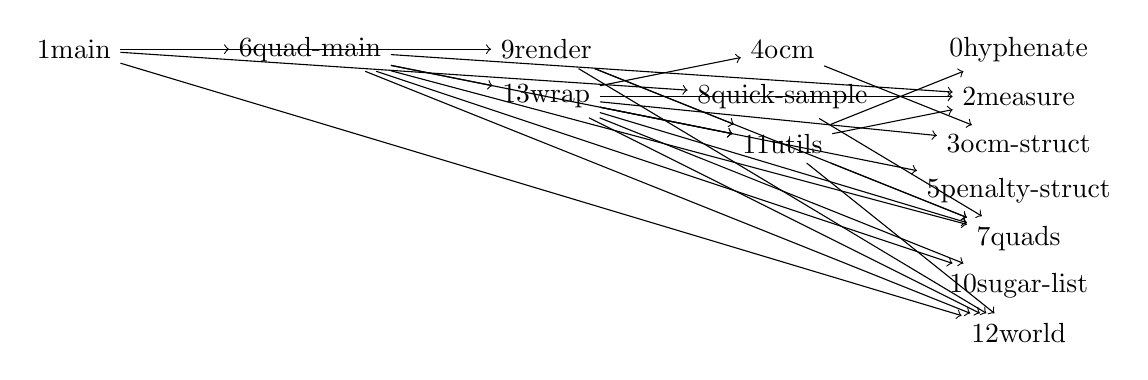
\begin{tikzpicture}

  \node (00)  {\rkt{0}{hyphenate}};
  \node (01) [below of=00,yshift=0.4cm] {\rkt{2}{measure}};
  \node (02) [below of=01,yshift=0.4cm] {\rkt{3}{ocm-struct}};
  \node (03) [below of=02,yshift=0.4cm] {\rkt{5}{penalty-struct}};
  \node (04) [below of=03,yshift=0.4cm] {\rkt{7}{quads}};
  \node (05) [below of=04,yshift=0.4cm] {\rkt{10}{sugar-list}};
  \node (06) [below of=05,yshift=0.4cm] {\rkt{12}{world}};
  \node (10) [left of=00,xshift=-2cm] {\rkt{4}{ocm}};
  \node (11) [below of=10,yshift=0.4cm] {\rkt{8}{quick-sample}};
  \node (12) [below of=11,yshift=0.4cm] {\rkt{11}{utils}};
  \node (20) [left of=10,xshift=-2cm] {\rkt{9}{render}};
  \node (21) [below of=20,yshift=0.4cm] {\rkt{13}{wrap}};
  \node (30) [left of=20,xshift=-2cm] {\rkt{6}{quad-main}};
  \node (40) [left of=30,xshift=-2cm] {\rkt{1}{main}};

  \draw[->] (10) -- (02);
  \draw[->] (11) -- (04);
  \draw[->] (12) -- (06);
  \draw[->] (12) -- (04);
  \draw[->] (12) -- (01);
  \draw[->] (12) -- (00);
  \draw[->] (20) -- (04);
  \draw[->] (20) -- (12);
  \draw[->] (20) -- (06);
  \draw[->] (21) -- (05);
  \draw[->] (21) -- (10);
  \draw[->] (21) -- (12);
  \draw[->] (21) -- (06);
  \draw[->] (21) -- (04);
  \draw[->] (21) -- (01);
  \draw[->] (21) -- (03);
  \draw[->] (21) -- (02);
  \draw[->] (30) -- (05);
  \draw[->] (30) -- (12);
  \draw[->] (30) -- (01);
  \draw[->] (30) -- (06);
  \draw[->] (30) -- (21);
  \draw[->] (30) -- (04);
  \draw[->] (40) -- (20);
  \draw[->] (40) -- (11);
  \draw[->] (40) -- (30);
  \draw[->] (40) -- (06);

\end{tikzpicture}
